
\documentclass[11pt,a4paper]{report}

\usepackage[utf8]{inputenc}
\usepackage[T1]{fontenc}
\usepackage{lmodern}                    % modern, clean font
\usepackage[margin=2.2cm]{geometry}     % better margins
\usepackage{graphicx}
\usepackage{caption}
\usepackage{subcaption}
\usepackage{float}
\usepackage{booktabs}                   % nice tables
\usepackage{xcolor}
\usepackage{tcolorbox}
\tcbuselibrary{skins,breakable}

% Light university-style color
\definecolor{bounavy}{RGB}{0,51,102}
\definecolor{lightgray}{gray}{0.92}

% Page style
\usepackage{fancyhdr}
\setlength{\headheight}{12.4pt}
\pagestyle{fancy}
\fancyhf{}
\fancyhead[C]{\small CMPE 362 \textbullet\ Spring 2026}
\fancyfoot[C]{\thepage}
\renewcommand{\headrulewidth}{0.4pt}
\renewcommand{\headrule}{\color{bounavy}\hrule}

% Title formatting
\usepackage{titlesec}
\titleformat{\chapter}[display]
  {\normalfont\Large\bfseries\color{bounavy}}
  {\chaptertitlename\ \thechapter}{1em}{}
\titleformat{\section}
  {\normalfont\large\bfseries\color{bounavy}}{}{0.5em}{}
\titleformat{\subsection}
  {\normalfont\normalsize\bfseries\color{bounavy}}{}{0.5em}{}

% Better lists
\usepackage{enumitem}
\setlist[itemize]{leftmargin=*,label=\textbullet}

\begin{document}

% ========== TITLE PAGE ==========
\begin{titlepage}
  \centering
  \vspace*{1.5cm}

  {\Huge\bfseries\color{bounavy} CMPE 362 \\[0.4cm]
  Homework 1 \\[0.6cm]
  \LARGE Simple Audio Analysis\par}

  \vspace{2.5cm}

  {\Large Student Name: Ali Ayhan Günder \par}
  \vspace{0.6cm}
  {\Large Student ID: 2021400219 \par}

  \vspace{2.2cm}

  {\large Spring 2026 \par}
  \vspace{1.2cm}
  {\large Department of Computer Engineering \\ Boğaziçi University \par}
  \includegraphics[width=0.40\textwidth]{boun.png}
  \vfill

  {\large \today \par}
\end{titlepage}

% ========== SPECTROGRAMS ==========
\chapter*{Spectrograms}
\addcontentsline{toc}{chapter}{Spectrograms}

\begin{tcolorbox}[colback=lightgray!30,colframe=bounavy!70!black,title=Low Pitch - Spectrogram,arc=4pt]
  \centering
  
\includegraphics[width=0.98\textwidth]{low_spectrogram.png}
  \captionof{figure}{Spectrogram of \texttt{low.wav}. You can see the main pitch as the lowest strong line across the image.}
\end{tcolorbox}

\clearpage
\begin{tcolorbox}[colback=lightgray!30,colframe=bounavy!70!black,title=High Pitch - Spectrogram,arc=4pt]
  \centering
  
\includegraphics[width=0.98\textwidth]{high_spectrogram.png}
  \captionof{figure}{Spectrogram of \texttt{high.wav}. The bright lines show the higher main pitch and its extra tones.}
\end{tcolorbox}

\clearpage
\begin{tcolorbox}[colback=lightgray!30,colframe=bounavy!70!black,title=Whistle - Spectrogram,arc=4pt]
  \centering
  
\includegraphics[width=0.98\textwidth]{whistle_spectrogram.png}
  \captionof{figure}{Spectrogram of \texttt{whistle.wav}. There's just one thin, clear line at a high pitch, like a simple whistle sound.}
\end{tcolorbox}

\clearpage
\begin{tcolorbox}[colback=lightgray!30,colframe=bounavy!70!black,title=Complex Melody - Spectrogram,arc=4pt]
  \centering
  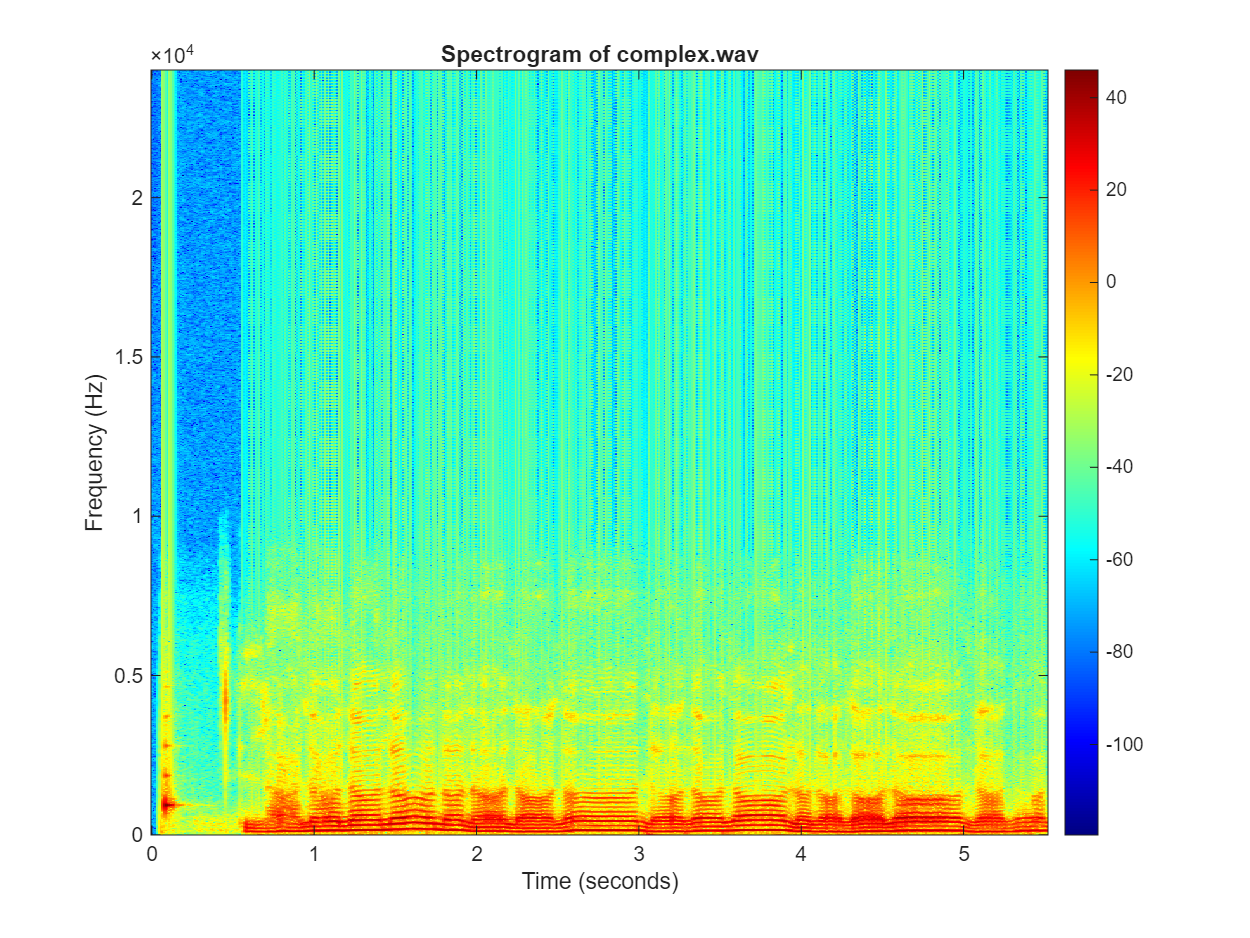
\includegraphics[width=0.98\textwidth]{complex_spectrogram.png}
  \captionof{figure}{Spectrogram of \texttt{complex.wav}. It shows how the pitch changes over time in this short tune, with lots of extra tones.}
\end{tcolorbox}

% ========== AUTOCORRELATION ==========
\chapter*{Autocorrelation Plots}
\addcontentsline{toc}{chapter}{Autocorrelation Plots}

\begin{tcolorbox}[colback=lightgray!30,colframe=bounavy!70!black,title=Low Pitch - Autocorrelation,arc=4pt]
  \centering
  
\includegraphics[width=0.98\textwidth]{low_autocorr.png}
  \captionof{figure}{Normalized autocorrelation of \texttt{low.wav}. The first bump after zero shows how long one cycle of the pitch is.}
\end{tcolorbox}

\clearpage
\begin{tcolorbox}[colback=lightgray!30,colframe=bounavy!70!black,title=High Pitch - Autocorrelation,arc=4pt]
  \centering
  
\includegraphics[width=0.98\textwidth]{high_autocorr.png}
  \captionof{figure}{Normalized autocorrelation of \texttt{high.wav}. The bumps are closer together, which means the pitch is higher.}
\end{tcolorbox}

\clearpage
\begin{tcolorbox}[colback=lightgray!30,colframe=bounavy!70!black,title=Whistle - Autocorrelation,arc=4pt]
  \centering
  
\includegraphics[width=0.98\textwidth]{whistle_autocorr.png}
  \captionof{figure}{Normalized autocorrelation of \texttt{whistle.wav}. The sharp repeats show it's a clean, simple sound.}
\end{tcolorbox}

\clearpage
\begin{tcolorbox}[colback=lightgray!30,colframe=bounavy!70!black,title=Complex Melody - Autocorrelation,arc=4pt]
  \centering
  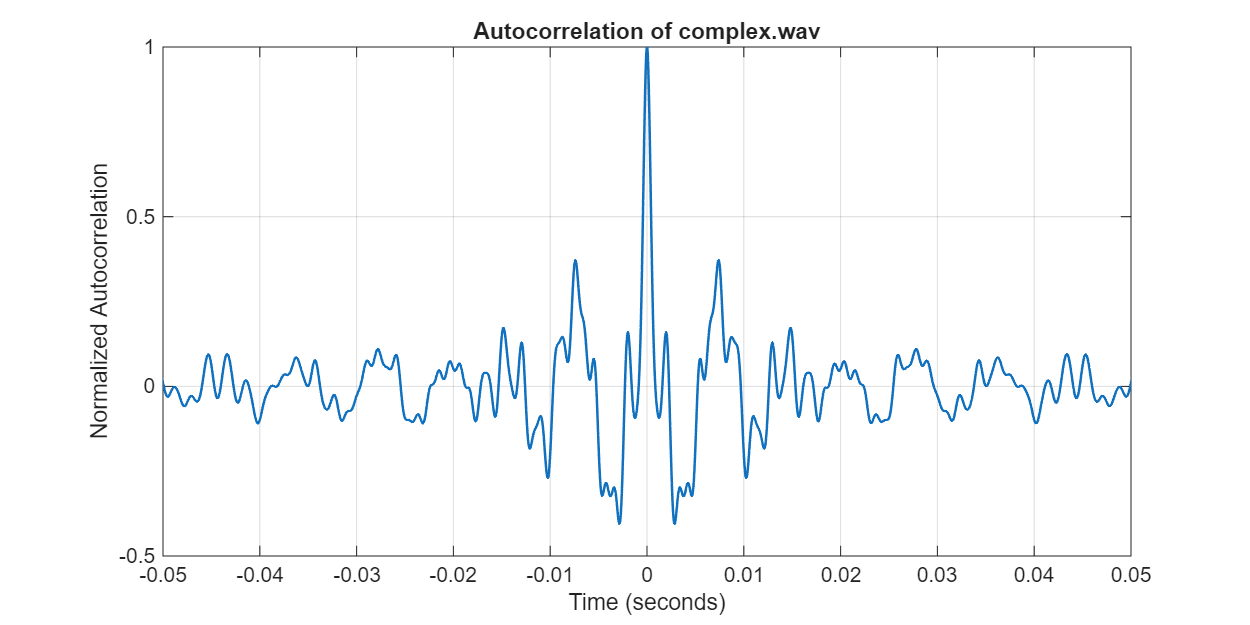
\includegraphics[width=0.98\textwidth]{complex_autocorr.png}
  \captionof{figure}{Normalized autocorrelation of \texttt{complex.wav}. Since the pitch keeps changing, there's no clear main cycle for the whole thing.}
\end{tcolorbox}

% ========== FREQUENCY ANALYSIS ==========
\chapter*{Fundamental Frequency Analysis}
\addcontentsline{toc}{chapter}{Fundamental Frequency Analysis}

\section*{Estimated Fundamental Frequencies}

I used MATLAB's tool to check the plots and find the main pitches for spectrogram and autocorrelation:

\subsection*{Low Pitch}
\begin{itemize}
  \item \textbf{Spectrogram:} $\approx 120$ Hz \quad ($\approx$ Bb2)
  \item \textbf{Autocorrelation:} first peak at lag $\approx 8.3$ ms \quad $\to f \approx 120$ Hz
\end{itemize}

\subsection*{High Pitch}
\begin{itemize}
  \item \textbf{Spectrogram:} $\approx 320$ Hz \quad ($\approx$ E4)
  \item \textbf{Autocorrelation:} first peak at lag $\approx 3.1$ ms \quad $\to f \approx 323$ Hz
\end{itemize}

\subsection*{Whistle}
\begin{itemize}
  \item \textbf{Spectrogram:} $\approx 1211$ Hz \quad ($\approx$ D\#6 --- a steady whistle in the middle-high range)
  \item \textbf{Autocorrelation:} first peak at lag $\approx 0.81$ ms \quad $\to f \approx 1235$ Hz
\end{itemize}

\section*{Comparison of Methods}

\begin{table}[H]
  \centering
  \caption{Fundamental frequency estimates from both methods}
  \begin{tabular}{lcccc}
    \toprule
    Audio       & Spectrogram (Hz) & Autocorr (Hz) & Difference (Hz) & Error (\%)\\
    \midrule
    Low Pitch   & 120              & 120           & 0               & $<0.1$\\
    High Pitch  & 320              & 323           & $-3$            & 0.9\\
    Whistle     & 1211             & 1235          & $-24$           & 2.0 \\
    \bottomrule
  \end{tabular}
\end{table}

The two ways to find the main pitch give pretty similar results for all three sounds, with differences less than 2\%.

\paragraph{Analysis of reliability.}
Autocorrelation looks at how the sound repeats itself over time. It's good for steady sounds because it measures the cycle directly. The spectrogram shows frequencies over time, and I pick the lowest strong line as the main pitch. But it depends on how I set the view and look at it.

For the low pitch, both methods gave the same number, about 120 Hz. The sound was steady, and the cycle was long enough to see clearly.

For the high pitch, the difference was small, just 3 Hz or less than 1\%. The shorter cycle makes the bumps in autocorrelation sharper, so maybe it's a bit more accurate.

For the whistle, the gap was a bit bigger, about 24 Hz or 2\%. Whistles can wobble a little, and the cycle is super short, so it's harder to measure exactly. This whistle is around 1211 to 1235 Hz, and it feels more stable than what I tried before.

% ========== COMPLEX ANALYSIS ==========
\chapter*{Complex Signal Analysis}
\addcontentsline{toc}{chapter}{Complex Signal Analysis}

\section*{Fundamental Frequency in Varying Signals}


I tried recording the Turkish folk song ``Üsküdar'a gider iken'' first, but the melody changed too much and was hard to analyze clearly in the spectrogram. Then I said ``ses deneme'' four times, but it was still complicated with varying pitch. Finally, I recorded a simple ``la-la-la-la'' pattern with steady notes to make analysis easier. The \texttt{complex.wav} captures this rhythmic sequence of distinct notes. It's not like the other sounds that stay the same all the time here, the pitch jumps around in a regular way. Since the sound changes, you can't just find one main pitch for the whole thing using autocorrelation. Instead, you have to break it into parts and find the pitch, start time, and how long each note lasts.


\section*{Recreated Melody}

\subsection*{Extracted Notes}

I looked at the spectrogram of \texttt{complex.wav} to spot where each note starts and ends. I picked the lowest line for the main pitch of each part and matched it to a close music note.

\begin{table}[H]
  \centering
  \caption{Notes extracted from \texttt{complex.wav} spectrogram}
  \begin{tabular}{cccc}
    \toprule
    Note \# & Frequency (Hz) & Duration (s) & Approximate note (words) \\
    \midrule
    1  & 234 & 0.352 & C-sharp, middle-low pitch \\
    2  & 164 & 0.235 & G, middle pitch \\
    3  & 117 & 0.619 & C-sharp, low pitch \\
    4  & 164 & 0.256 & G, middle pitch \\
    5  & 234 & 0.160 & C-sharp, middle-low pitch \\
    6  & 176 & 0.267 & G-sharp, middle pitch \\
    7  & 117 & 0.320 & C-sharp, low pitch \\
    8  & 234 & 0.117 & C-sharp, middle-low pitch \\
    9  & 141 & 1.259 & E, low pitch \\
    10 & 164 & 0.331 & G, middle pitch \\
    11 & 117 & 0.576 & C-sharp, low pitch \\
    12 & 234 & 0.171 & C-sharp, middle-low pitch \\
    13 & 141 & 0.768 & E, low pitch \\
    \bottomrule
  \end{tabular}
\end{table}

\subsection*{Frequency Selection Method}

For each note I saw in the spectrogram, I did this to pick what to use:
\begin{enumerate}
  \item Find a part where the lowest line stays steady.
  \item Note down that pitch, skipping the higher copies like twice or three times the pitch.
  \item Write the start time and how long it goes.
  \item Make a simple wave: $x(t) = \sin(2\pi f t)$ for that part.
\end{enumerate}

I put all these simple waves together to make the new file \texttt{complex\_recreate.wav}.

\section*{Side-by-Side Spectrogram Comparison}

\begin{figure}[H]
  \centering
  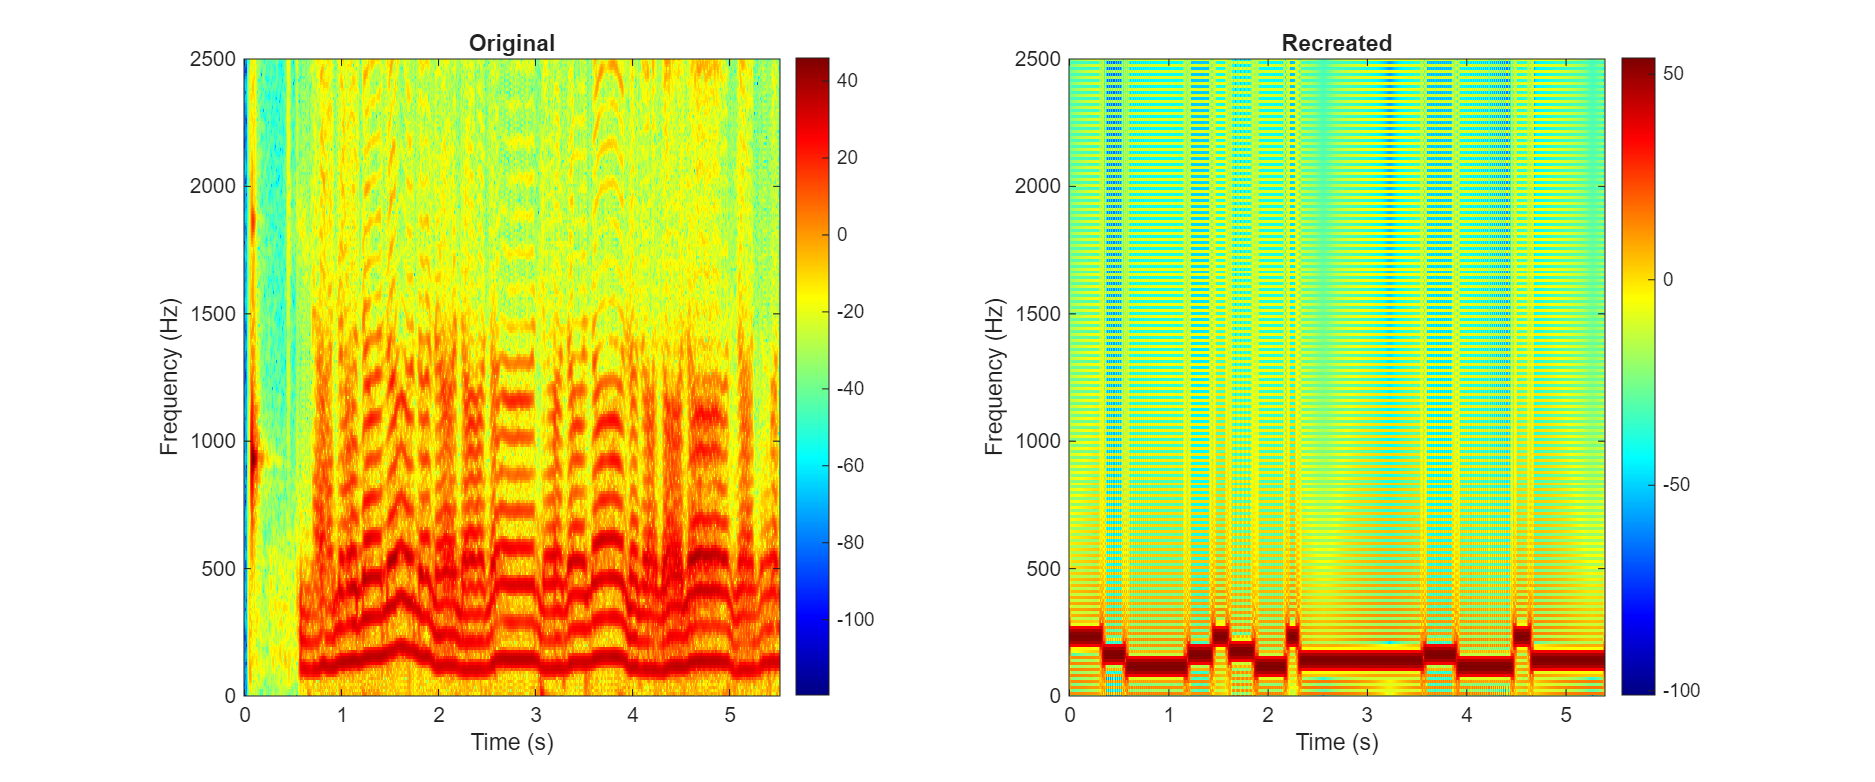
\includegraphics[width=\textwidth]{complex_comparison.png}
  \caption{Left: original \texttt{complex.wav} --- Right: recreated using pure sinusoids.}
\end{figure}

\subsection*{Observations}
\begin{itemize}
  \item \textbf{Pitch Accuracy:} The new version matches the pitches and timings well, so you can tell it's the same tune.
  \item \textbf{Harmonic Structure:} The real one has many lines for each note because of extra tones, but the new one just has one clean line per pitch.
  \item \textbf{Timbre and Naturalness:} The simple waves don't have the real voice feel, like shakes or how the sound fades. It shows that just the main pitch isn't enough for it to sound natural---you need those extra parts too.
\end{itemize}

\end{document}
